\chapter{Characterisation of the downstream time of flight system}
\label{ch:hptpc_dtof_characterisation}

The time taken by a particle to traverse a distance $L$ is given by
\begin{equation}
  t = L \sqrt{ \frac{m^{2}}{p^{2}} + \frac{1}{c^{2}} } \, ,
\end{equation}
where $m$ is the mass of the particle, $p$ is the particle momentum and $c$ is the speed of light in a vacuum.

\citesec{ch:hptpc_dtof_characterisation:dtof} describes the DToF while \citesec{ch:hptpc_dtof_characterisation:characterisation} describes the characterisation of the PMTs and bars.

\section{The downstream time of flight system (DToF)}
\label{ch:hptpc_dtof_characterisation:dtof}

The DToF consists of 10 bars made up of Nuvia NuDET plastic scintillator which has a wavelength of maximum emission of \SI{425}{\milli\metre} and a decay time constant of \SI{2.5}{\nano\second}~\cite{nuvia}.
Each one of these bars measures $\SI{10}{\centi\metre} \times \SI{1}{\centi\metre} \times \SI{140}{\centi\metre}$.
A diagram of one such bar is shown in \citefig{fig:barDiag}.
The curved cutouts at either end of the bar each accomodate a 5'' Hamamatsu Photonics R6594 PMT~\cite{hamamatsu}.

\begin{figure}
  \centering
  \includegraphics[width=.8\linewidth]{files/figures/hptpc_dtof_characterisation/barDiag}
  \caption[HPTPC DToF bar diagram]{Computer generated drawing of one of the scintillator bars from two views.}
  \label{fig:barDiag}
\end{figure}

The bars and PMTs are arranged in two rows of five bars to ensure complete coverage for any particles impinging on the detector.
This gives the DToF a total active area of $\SI{1.40}{\metre} \times \SI{0.78}{\metre}$.
\citefig{fig:dtofDiag} shows a diagram of the DToF system along with various dimensions of sections of the detector.
Each of the bars is wrapped individually in a reflective milar sheet in order to maximise the light yield as well as keeping external light out of the bar.

\begin{figure}[h]
  \centering
  \includegraphics[width=.5\linewidth]{files/figures/hptpc_dtof_characterisation/dstofFront}
  \caption[Diagram of the HPTPC DToF]{Diagram of the DToF along with measurements.}
  \label{fig:dtofDiag}
\end{figure}

Each of the PMTs is attached to the scintillator bar via 3D-printed support which is glued to the bar.
A layer of optical grease is applied to the end of the scintillator bar where it meets the PMT.
This ensures good optical coupling between the PMT and scintillator bar and minimises light loss.

The vertical position of a particle striking the DToF can be measured by observing in which bar a signal is observed.
The horizontal position of the same particle can be inferred by measuring the time difference between signals being observed in PMTs at opposite ends of the same bar.

However, in order to effectively convert this time measurement to one of position, two factors must be measured.
Firstly, the relationship between the time difference in signals being observed in PMTs and the position of a particle along the bar must be measured.
Secondly, the time (and therefore position) resolution must be measured.
The procedure and results of these measurements are discussed in \citesec{ch:hptpc_dtof_characterisation:characterisation}.

\section{Characterisation of the bars}
\label{ch:hptpc_dtof_characterisation:characterisation}

\subsection{PMT characterisation}
\label{ch:hptpc_dtof_characterisation:characterisation:pmt}

Prior to testing the bars with the PMTs attached, the gains of each PMT are measured.
This is done in order to determine where to place each PMT within the detector.
A PMT with a higher gain will have a higher light collection efficiency and so will be more likely to deetect light from a given charged particle.
These higher gain PMTs are attached to the bars upon which the beam centre impinges and so will observe the highest flux of particles.

The gain of a PMT can be expressed as
\begin{equation}
  G = \frac{N_{\text{SE}}}{N_{\text{PE}}} \, ,
\end{equation}
where $N_{\text{SE}}$ is the number of output signal electrons and $N_{\text{PE}}$ is the number of photoelectrons liberated from the photocathode.
This gain measurement is performed by pulsing an LED lamp directly into the photocathode of each PMT with the same voltage used for each LED pulse.
The output waveform produced by the PMT is then read by an oscilloscope.

$N_{\text{SE}}$ can be determined from the output PMT waveform in the following manner.
This waveform is in voltage units and can be converted to current by dividing by the resistance of the oscilloscope.
The relationship between charge, $Q$, and current, $I$, is given by
\begin{equation}
  Q = \int I(t) \, dt
\end{equation}
where $Q$ is in coulombs, $I$ is amperes and $t$ is in seconds.
Therefore, $N_{\text{SE}}$ can be expressed as
\begin{equation}
  N_{\text{SE}} = \frac{1}{R q_{e}} \int V(t) \, dt
\end{equation}
where $q_{e}$ is the elementary charge.
This process is then repeated a number of times.
An example of the gaussian distribution produced from a number of waveforms is shown in \citefig{fig:N_se}.

\begin{figure}[h]
  \begin{adjustbox}{max totalsize={\textwidth}, center}
    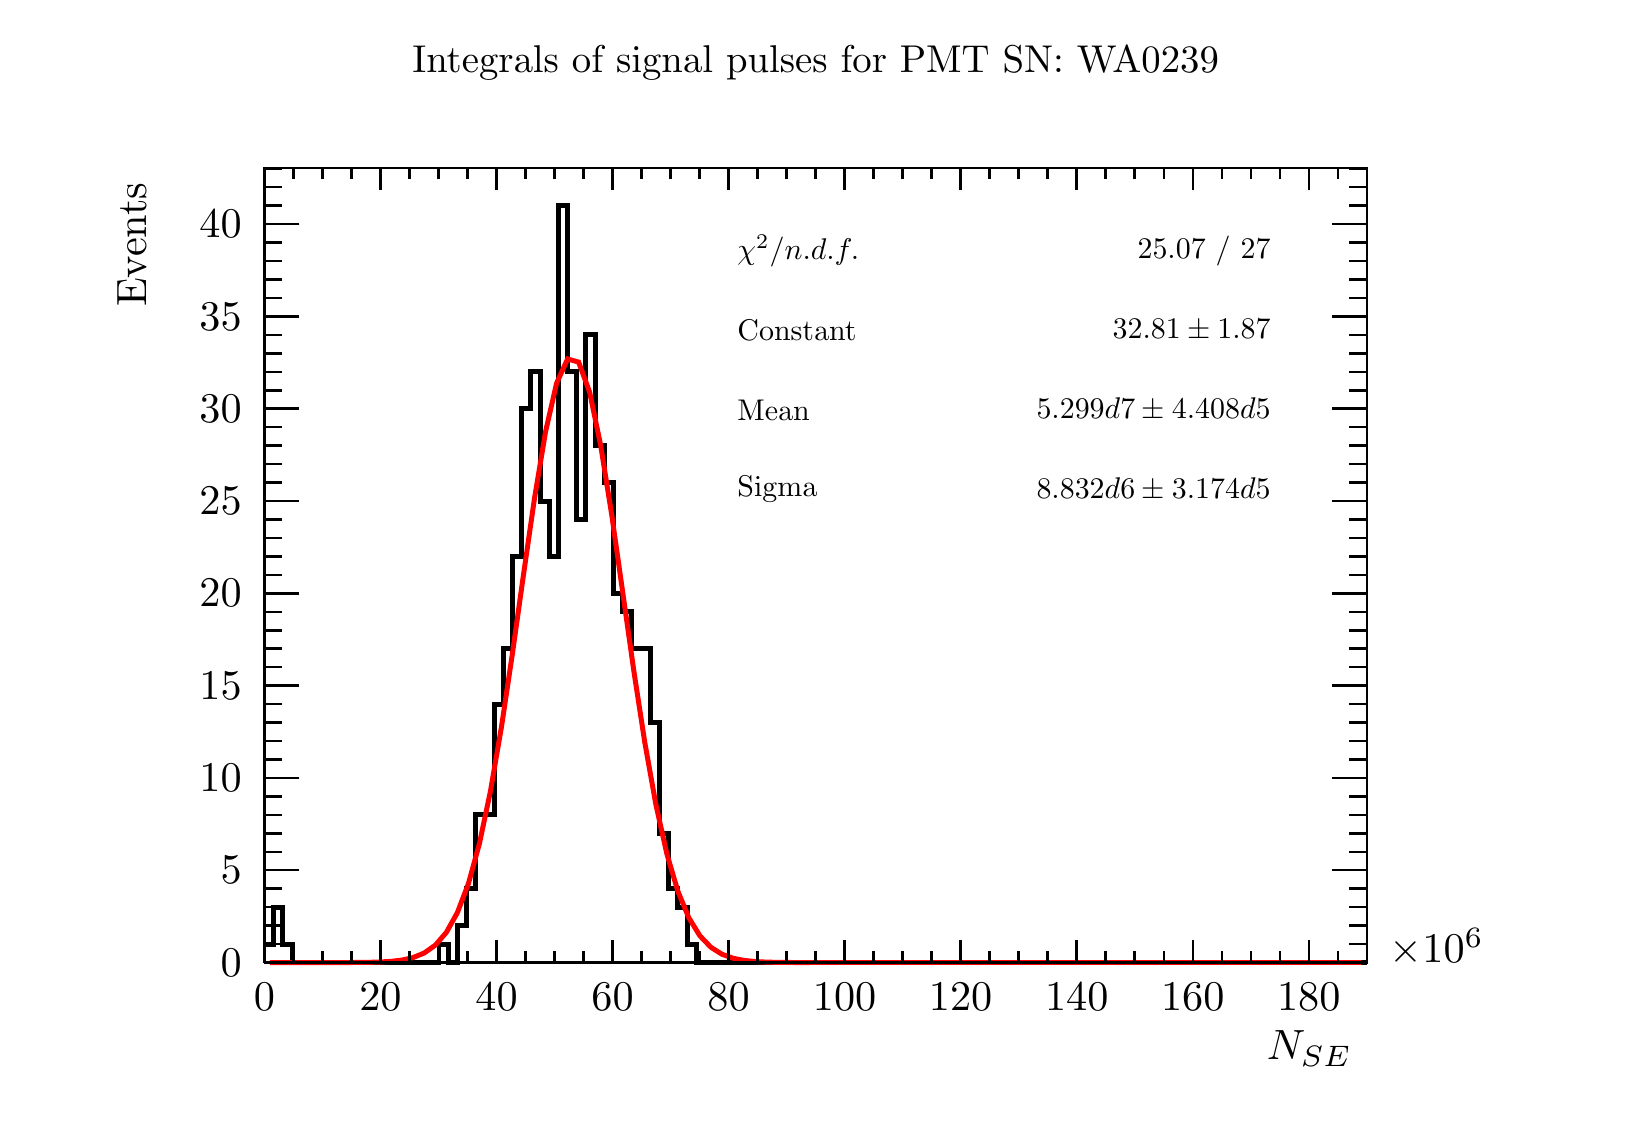
\begin{tikzpicture}
\pgfdeclareplotmark{cross} {
\pgfpathmoveto{\pgfpoint{-0.3\pgfplotmarksize}{\pgfplotmarksize}}
\pgfpathlineto{\pgfpoint{+0.3\pgfplotmarksize}{\pgfplotmarksize}}
\pgfpathlineto{\pgfpoint{+0.3\pgfplotmarksize}{0.3\pgfplotmarksize}}
\pgfpathlineto{\pgfpoint{+1\pgfplotmarksize}{0.3\pgfplotmarksize}}
\pgfpathlineto{\pgfpoint{+1\pgfplotmarksize}{-0.3\pgfplotmarksize}}
\pgfpathlineto{\pgfpoint{+0.3\pgfplotmarksize}{-0.3\pgfplotmarksize}}
\pgfpathlineto{\pgfpoint{+0.3\pgfplotmarksize}{-1.\pgfplotmarksize}}
\pgfpathlineto{\pgfpoint{-0.3\pgfplotmarksize}{-1.\pgfplotmarksize}}
\pgfpathlineto{\pgfpoint{-0.3\pgfplotmarksize}{-0.3\pgfplotmarksize}}
\pgfpathlineto{\pgfpoint{-1.\pgfplotmarksize}{-0.3\pgfplotmarksize}}
\pgfpathlineto{\pgfpoint{-1.\pgfplotmarksize}{0.3\pgfplotmarksize}}
\pgfpathlineto{\pgfpoint{-0.3\pgfplotmarksize}{0.3\pgfplotmarksize}}
\pgfpathclose
\pgfusepathqstroke
}
\pgfdeclareplotmark{cross*} {
\pgfpathmoveto{\pgfpoint{-0.3\pgfplotmarksize}{\pgfplotmarksize}}
\pgfpathlineto{\pgfpoint{+0.3\pgfplotmarksize}{\pgfplotmarksize}}
\pgfpathlineto{\pgfpoint{+0.3\pgfplotmarksize}{0.3\pgfplotmarksize}}
\pgfpathlineto{\pgfpoint{+1\pgfplotmarksize}{0.3\pgfplotmarksize}}
\pgfpathlineto{\pgfpoint{+1\pgfplotmarksize}{-0.3\pgfplotmarksize}}
\pgfpathlineto{\pgfpoint{+0.3\pgfplotmarksize}{-0.3\pgfplotmarksize}}
\pgfpathlineto{\pgfpoint{+0.3\pgfplotmarksize}{-1.\pgfplotmarksize}}
\pgfpathlineto{\pgfpoint{-0.3\pgfplotmarksize}{-1.\pgfplotmarksize}}
\pgfpathlineto{\pgfpoint{-0.3\pgfplotmarksize}{-0.3\pgfplotmarksize}}
\pgfpathlineto{\pgfpoint{-1.\pgfplotmarksize}{-0.3\pgfplotmarksize}}
\pgfpathlineto{\pgfpoint{-1.\pgfplotmarksize}{0.3\pgfplotmarksize}}
\pgfpathlineto{\pgfpoint{-0.3\pgfplotmarksize}{0.3\pgfplotmarksize}}
\pgfpathclose
\pgfusepathqfillstroke
}
\pgfdeclareplotmark{newstar} {
\pgfpathmoveto{\pgfqpoint{0pt}{\pgfplotmarksize}}
\pgfpathlineto{\pgfqpointpolar{44}{0.5\pgfplotmarksize}}
\pgfpathlineto{\pgfqpointpolar{18}{\pgfplotmarksize}}
\pgfpathlineto{\pgfqpointpolar{-20}{0.5\pgfplotmarksize}}
\pgfpathlineto{\pgfqpointpolar{-54}{\pgfplotmarksize}}
\pgfpathlineto{\pgfqpointpolar{-90}{0.5\pgfplotmarksize}}
\pgfpathlineto{\pgfqpointpolar{234}{\pgfplotmarksize}}
\pgfpathlineto{\pgfqpointpolar{198}{0.5\pgfplotmarksize}}
\pgfpathlineto{\pgfqpointpolar{162}{\pgfplotmarksize}}
\pgfpathlineto{\pgfqpointpolar{134}{0.5\pgfplotmarksize}}
\pgfpathclose
\pgfusepathqstroke
}
\pgfdeclareplotmark{newstar*} {
\pgfpathmoveto{\pgfqpoint{0pt}{\pgfplotmarksize}}
\pgfpathlineto{\pgfqpointpolar{44}{0.5\pgfplotmarksize}}
\pgfpathlineto{\pgfqpointpolar{18}{\pgfplotmarksize}}
\pgfpathlineto{\pgfqpointpolar{-20}{0.5\pgfplotmarksize}}
\pgfpathlineto{\pgfqpointpolar{-54}{\pgfplotmarksize}}
\pgfpathlineto{\pgfqpointpolar{-90}{0.5\pgfplotmarksize}}
\pgfpathlineto{\pgfqpointpolar{234}{\pgfplotmarksize}}
\pgfpathlineto{\pgfqpointpolar{198}{0.5\pgfplotmarksize}}
\pgfpathlineto{\pgfqpointpolar{162}{\pgfplotmarksize}}
\pgfpathlineto{\pgfqpointpolar{134}{0.5\pgfplotmarksize}}
\pgfpathclose
\pgfusepathqfillstroke
}
\definecolor{c}{rgb}{1,1,1};
\draw [color=c, fill=c] (0,0) rectangle (20,13.639);
\draw [color=c, fill=c] (3,1.77307) rectangle (17,11.8659);
\definecolor{c}{rgb}{0,0,0};
\draw [c,line width=0.9] (3,1.77307) -- (3,11.8659) -- (17,11.8659) -- (17,1.77307) -- (3,1.77307);
\definecolor{c}{rgb}{1,1,1};
\draw [color=c, fill=c] (3,1.77307) rectangle (17,11.8659);
\definecolor{c}{rgb}{0,0,0};
\draw [c,line width=0.9] (3,1.77307) -- (3,11.8659) -- (17,11.8659) -- (17,1.77307) -- (3,1.77307);
\draw [c,line width=1.8] (3,2.00751) -- (3.11667,2.00751) -- (3.11667,2.4764) -- (3.23333,2.4764) -- (3.23333,2.00751) -- (3.35,2.00751) -- (3.35,1.77307) -- (3.46667,1.77307) -- (3.46667,1.77307) -- (3.58333,1.77307) -- (3.58333,1.77307) --
 (3.7,1.77307) -- (3.7,1.77307) -- (3.81667,1.77307) -- (3.81667,1.77307) -- (3.93333,1.77307) -- (3.93333,1.77307) -- (4.05,1.77307) -- (4.05,1.77307) -- (4.16667,1.77307) -- (4.16667,1.77307) -- (4.28333,1.77307) -- (4.28333,1.77307) --
 (4.4,1.77307) -- (4.4,1.77307) -- (4.51667,1.77307) -- (4.51667,1.77307) -- (4.63333,1.77307) -- (4.63333,1.77307) -- (4.75,1.77307) -- (4.75,1.77307) -- (4.86667,1.77307) -- (4.86667,1.77307) -- (4.98333,1.77307) -- (4.98333,1.77307) --
 (5.1,1.77307) -- (5.1,1.77307) -- (5.21667,1.77307) -- (5.21667,2.00751) -- (5.33333,2.00751) -- (5.33333,1.77307) -- (5.45,1.77307) -- (5.45,2.24195) -- (5.56667,2.24195) -- (5.56667,2.71084) -- (5.68333,2.71084) -- (5.68333,3.64862) --
 (5.8,3.64862) -- (5.8,3.64862) -- (5.91667,3.64862) -- (5.91667,5.05529) -- (6.03333,5.05529) -- (6.03333,5.75862) -- (6.15,5.75862) -- (6.15,6.93085) -- (6.26667,6.93085) -- (6.26667,8.8064) -- (6.38333,8.8064) -- (6.38333,9.27529) -- (6.5,9.27529)
 -- (6.5,7.63418) -- (6.61667,7.63418) -- (6.61667,6.93085) -- (6.73333,6.93085) -- (6.73333,11.3853) -- (6.85,11.3853) -- (6.85,9.27529) -- (6.96667,9.27529) -- (6.96667,7.39973) -- (7.08333,7.39973) -- (7.08333,9.74418) -- (7.2,9.74418) --
 (7.2,8.33751) -- (7.31667,8.33751) -- (7.31667,7.86862) -- (7.43333,7.86862) -- (7.43333,6.46196) -- (7.55,6.46196) -- (7.55,6.22751) -- (7.66667,6.22751) -- (7.66667,5.75862) -- (7.78333,5.75862) -- (7.78333,5.75862) -- (7.9,5.75862) --
 (7.9,4.82084) -- (8.01667,4.82084) -- (8.01667,3.41418) -- (8.13333,3.41418) -- (8.13333,2.71084) -- (8.25,2.71084) -- (8.25,2.4764) -- (8.36667,2.4764) -- (8.36667,2.00751) -- (8.48333,2.00751) -- (8.48333,1.77307) -- (8.6,1.77307) -- (8.6,1.77307)
 -- (8.71667,1.77307) -- (8.71667,1.77307) -- (8.83333,1.77307) -- (8.83333,1.77307) -- (8.95,1.77307) -- (8.95,1.77307) -- (9.06667,1.77307) -- (9.06667,1.77307) -- (9.18333,1.77307) -- (9.18333,1.77307) -- (9.3,1.77307) -- (9.3,1.77307) --
 (9.41667,1.77307) -- (9.41667,1.77307) -- (9.53333,1.77307) -- (9.53333,1.77307) -- (9.65,1.77307) -- (9.65,1.77307) -- (9.76667,1.77307) -- (9.76667,1.77307) -- (9.88333,1.77307) -- (9.88333,1.77307) -- (10,1.77307) -- (10,1.77307) --
 (10.1167,1.77307) -- (10.1167,1.77307) -- (10.2333,1.77307) -- (10.2333,1.77307) -- (10.35,1.77307) -- (10.35,1.77307) -- (10.4667,1.77307) -- (10.4667,1.77307) -- (10.5833,1.77307) -- (10.5833,1.77307) -- (10.7,1.77307) -- (10.7,1.77307) --
 (10.8167,1.77307) -- (10.8167,1.77307) -- (10.9333,1.77307) -- (10.9333,1.77307) -- (11.05,1.77307) -- (11.05,1.77307) -- (11.1667,1.77307) -- (11.1667,1.77307) -- (11.2833,1.77307) -- (11.2833,1.77307) -- (11.4,1.77307) -- (11.4,1.77307) --
 (11.5167,1.77307) -- (11.5167,1.77307) -- (11.6333,1.77307) -- (11.6333,1.77307) -- (11.75,1.77307) -- (11.75,1.77307) -- (11.8667,1.77307) -- (11.8667,1.77307) -- (11.9833,1.77307) -- (11.9833,1.77307) -- (12.1,1.77307) -- (12.1,1.77307) --
 (12.2167,1.77307) -- (12.2167,1.77307) -- (12.3333,1.77307) -- (12.3333,1.77307) -- (12.45,1.77307) -- (12.45,1.77307) -- (12.5667,1.77307) -- (12.5667,1.77307) -- (12.6833,1.77307) -- (12.6833,1.77307) -- (12.8,1.77307) -- (12.8,1.77307) --
 (12.9167,1.77307) -- (12.9167,1.77307) -- (13.0333,1.77307) -- (13.0333,1.77307) -- (13.15,1.77307) -- (13.15,1.77307) -- (13.2667,1.77307) -- (13.2667,1.77307) -- (13.3833,1.77307) -- (13.3833,1.77307) -- (13.5,1.77307) -- (13.5,1.77307) --
 (13.6167,1.77307) -- (13.6167,1.77307) -- (13.7333,1.77307) -- (13.7333,1.77307) -- (13.85,1.77307) -- (13.85,1.77307) -- (13.9667,1.77307) -- (13.9667,1.77307) -- (14.0833,1.77307) -- (14.0833,1.77307) -- (14.2,1.77307) -- (14.2,1.77307) --
 (14.3167,1.77307) -- (14.3167,1.77307) -- (14.4333,1.77307) -- (14.4333,1.77307) -- (14.55,1.77307) -- (14.55,1.77307) -- (14.6667,1.77307) -- (14.6667,1.77307) -- (14.7833,1.77307) -- (14.7833,1.77307) -- (14.9,1.77307) -- (14.9,1.77307) --
 (15.0167,1.77307) -- (15.0167,1.77307) -- (15.1333,1.77307) -- (15.1333,1.77307) -- (15.25,1.77307) -- (15.25,1.77307) -- (15.3667,1.77307) -- (15.3667,1.77307) -- (15.4833,1.77307) -- (15.4833,1.77307) -- (15.6,1.77307) -- (15.6,1.77307) --
 (15.7167,1.77307) -- (15.7167,1.77307) -- (15.8333,1.77307) -- (15.8333,1.77307) -- (15.95,1.77307) -- (15.95,1.77307) -- (16.0667,1.77307) -- (16.0667,1.77307) -- (16.1833,1.77307) -- (16.1833,1.77307) -- (16.3,1.77307) -- (16.3,1.77307) --
 (16.4167,1.77307) -- (16.4167,1.77307) -- (16.5333,1.77307) -- (16.5333,1.77307) -- (16.65,1.77307) -- (16.65,1.77307) -- (16.7667,1.77307) -- (16.7667,1.77307) -- (16.8833,1.77307) -- (16.8833,1.77307) -- (17,1.77307);
\definecolor{c}{rgb}{1,0,0};
\draw [c,line width=1.8] (3.07,1.77307) -- (3.21,1.77307) -- (3.35,1.77307) -- (3.49,1.77307) -- (3.63,1.77307) -- (3.77,1.77307) -- (3.91,1.77307) -- (4.05,1.77307) -- (4.19,1.77435) -- (4.33,1.77614) -- (4.47,1.78011) -- (4.61,1.78845) --
 (4.75,1.80517) -- (4.89,1.837) -- (5.03,1.89465) -- (5.17,1.99382) -- (5.31,2.15575) -- (5.45,2.40645) -- (5.59,2.77398) -- (5.73,3.28325) -- (5.87,3.9486) -- (6.01,4.76533) -- (6.15,5.70256) -- (6.29,6.69998) -- (6.43,7.67119) -- (6.57,8.51452) --
 (6.71,9.12997) -- (6.85,9.43852) -- (6.99,9.3988) -- (7.13,9.0162) -- (7.27,8.34167) -- (7.41,7.46056) -- (7.55,6.47492) -- (7.69,5.48431) -- (7.83,4.56993) -- (7.97,3.78551) -- (8.11,3.1556) -- (8.25,2.67991) -- (8.39,2.34099) -- (8.53,2.11265) --
 (8.67,1.96693) -- (8.81,1.87874) -- (8.95,1.82806) -- (9.09,1.80039) -- (9.23,1.78603) -- (9.37,1.77894) -- (9.51,1.77561) -- (9.65,1.77411) -- (9.79,1.77307) -- (9.93,1.77307);
\draw [c,line width=1.8] (9.93,1.77307) -- (10.07,1.77307) -- (10.21,1.77307) -- (10.35,1.77307) -- (10.49,1.77307) -- (10.63,1.77307) -- (10.77,1.77307) -- (10.91,1.77307) -- (11.05,1.77307) -- (11.19,1.77307) -- (11.33,1.77307) -- (11.47,1.77307)
 -- (11.61,1.77307) -- (11.75,1.77307) -- (11.89,1.77307) -- (12.03,1.77307) -- (12.17,1.77307) -- (12.31,1.77307) -- (12.45,1.77307) -- (12.59,1.77307) -- (12.73,1.77307) -- (12.87,1.77307) -- (13.01,1.77307) -- (13.15,1.77307) -- (13.29,1.77307) --
 (13.43,1.77307) -- (13.57,1.77307) -- (13.71,1.77307) -- (13.85,1.77307) -- (13.99,1.77307) -- (14.13,1.77307) -- (14.27,1.77307) -- (14.41,1.77307) -- (14.55,1.77307) -- (14.69,1.77307) -- (14.83,1.77307) -- (14.97,1.77307) -- (15.11,1.77307) --
 (15.25,1.77307) -- (15.39,1.77307) -- (15.53,1.77307) -- (15.67,1.77307) -- (15.81,1.77307) -- (15.95,1.77307) -- (16.09,1.77307) -- (16.23,1.77307) -- (16.37,1.77307) -- (16.51,1.77307) -- (16.65,1.77307) -- (16.79,1.77307);
\draw [c,line width=1.8] (16.79,1.77307) -- (16.93,1.77307);
\definecolor{c}{rgb}{1,1,1};
\draw [color=c, fill=c] (8.48138,7.27794) rectangle (16.3037,11.3181);
\definecolor{c}{rgb}{0,0,0};
\draw [anchor= west] (8.87249,10.813) node[scale=1.08185, color=c, rotate=0]{$\chi^{2} / \text{n.d.f.} $};
\draw [anchor= east] (15.9126,10.813) node[scale=1.08185, color=c, rotate=0]{ 25.07 / 27};
\draw [anchor= west] (8.87249,9.80301) node[scale=1.08185, color=c, rotate=0]{Constant };
\draw [anchor= east] (15.9126,9.80301) node[scale=1.08185, color=c, rotate=0]{$ 32.81 \pm 1.87$};
\draw [anchor= west] (8.87249,8.79298) node[scale=1.08185, color=c, rotate=0]{Mean     };
\draw [anchor= east] (15.9126,8.79298) node[scale=1.08185, color=c, rotate=0]{$ \num{5.299d7} \pm \num{4.408d5}$};
\draw [anchor= west] (8.87249,7.78295) node[scale=1.08185, color=c, rotate=0]{Sigma    };
\draw [anchor= east] (15.9126,7.78295) node[scale=1.08185, color=c, rotate=0]{$ \num{8.832d6} \pm \num{3.174d5}$};
\draw [c,line width=0.9] (3,1.77307) -- (17,1.77307);
\draw [c,line width=0.9] (3,2.05948) -- (3,1.77307);
\draw [c,line width=0.9] (3.36842,1.91628) -- (3.36842,1.77307);
\draw [c,line width=0.9] (3.73684,1.91628) -- (3.73684,1.77307);
\draw [c,line width=0.9] (4.10526,1.91628) -- (4.10526,1.77307);
\draw [c,line width=0.9] (4.47368,2.05948) -- (4.47368,1.77307);
\draw [c,line width=0.9] (4.8421,1.91628) -- (4.8421,1.77307);
\draw [c,line width=0.9] (5.21053,1.91628) -- (5.21053,1.77307);
\draw [c,line width=0.9] (5.57895,1.91628) -- (5.57895,1.77307);
\draw [c,line width=0.9] (5.94737,2.05948) -- (5.94737,1.77307);
\draw [c,line width=0.9] (6.31579,1.91628) -- (6.31579,1.77307);
\draw [c,line width=0.9] (6.68421,1.91628) -- (6.68421,1.77307);
\draw [c,line width=0.9] (7.05263,1.91628) -- (7.05263,1.77307);
\draw [c,line width=0.9] (7.42105,2.05948) -- (7.42105,1.77307);
\draw [c,line width=0.9] (7.78947,1.91628) -- (7.78947,1.77307);
\draw [c,line width=0.9] (8.1579,1.91628) -- (8.1579,1.77307);
\draw [c,line width=0.9] (8.52632,1.91628) -- (8.52632,1.77307);
\draw [c,line width=0.9] (8.89474,2.05948) -- (8.89474,1.77307);
\draw [c,line width=0.9] (9.26316,1.91628) -- (9.26316,1.77307);
\draw [c,line width=0.9] (9.63158,1.91628) -- (9.63158,1.77307);
\draw [c,line width=0.9] (10,1.91628) -- (10,1.77307);
\draw [c,line width=0.9] (10.3684,2.05948) -- (10.3684,1.77307);
\draw [c,line width=0.9] (10.7368,1.91628) -- (10.7368,1.77307);
\draw [c,line width=0.9] (11.1053,1.91628) -- (11.1053,1.77307);
\draw [c,line width=0.9] (11.4737,1.91628) -- (11.4737,1.77307);
\draw [c,line width=0.9] (11.8421,2.05948) -- (11.8421,1.77307);
\draw [c,line width=0.9] (12.2105,1.91628) -- (12.2105,1.77307);
\draw [c,line width=0.9] (12.5789,1.91628) -- (12.5789,1.77307);
\draw [c,line width=0.9] (12.9474,1.91628) -- (12.9474,1.77307);
\draw [c,line width=0.9] (13.3158,2.05948) -- (13.3158,1.77307);
\draw [c,line width=0.9] (13.6842,1.91628) -- (13.6842,1.77307);
\draw [c,line width=0.9] (14.0526,1.91628) -- (14.0526,1.77307);
\draw [c,line width=0.9] (14.4211,1.91628) -- (14.4211,1.77307);
\draw [c,line width=0.9] (14.7895,2.05948) -- (14.7895,1.77307);
\draw [c,line width=0.9] (15.1579,1.91628) -- (15.1579,1.77307);
\draw [c,line width=0.9] (15.5263,1.91628) -- (15.5263,1.77307);
\draw [c,line width=0.9] (15.8947,1.91628) -- (15.8947,1.77307);
\draw [c,line width=0.9] (16.2632,2.05948) -- (16.2632,1.77307);
\draw [c,line width=0.9] (16.2632,2.05948) -- (16.2632,1.77307);
\draw [c,line width=0.9] (16.6316,1.91628) -- (16.6316,1.77307);
\draw [anchor=base] (3,1.15931) node[scale=1.52731, color=c, rotate=0]{0};
\draw [anchor=base] (4.47368,1.15931) node[scale=1.52731, color=c, rotate=0]{20};
\draw [anchor=base] (5.94737,1.15931) node[scale=1.52731, color=c, rotate=0]{40};
\draw [anchor=base] (7.42105,1.15931) node[scale=1.52731, color=c, rotate=0]{60};
\draw [anchor=base] (8.89474,1.15931) node[scale=1.52731, color=c, rotate=0]{80};
\draw [anchor=base] (10.3684,1.15931) node[scale=1.52731, color=c, rotate=0]{100};
\draw [anchor=base] (11.8421,1.15931) node[scale=1.52731, color=c, rotate=0]{120};
\draw [anchor=base] (13.3158,1.15931) node[scale=1.52731, color=c, rotate=0]{140};
\draw [anchor=base] (14.7895,1.15931) node[scale=1.52731, color=c, rotate=0]{160};
\draw [anchor=base] (16.2632,1.15931) node[scale=1.52731, color=c, rotate=0]{180};
\draw [anchor=base west] (17.1,1.77307) node[scale=1.52731, color=c, rotate=0]{$\times10^{6}$};
\draw [anchor= east] (17,0.681948) node[scale=1.52731, color=c, rotate=0]{$N_{\text{SE}}$};
\draw [c,line width=0.9] (3,11.8659) -- (17,11.8659);
\draw [c,line width=0.9] (3,11.5795) -- (3,11.8659);
\draw [c,line width=0.9] (3.36842,11.7227) -- (3.36842,11.8659);
\draw [c,line width=0.9] (3.73684,11.7227) -- (3.73684,11.8659);
\draw [c,line width=0.9] (4.10526,11.7227) -- (4.10526,11.8659);
\draw [c,line width=0.9] (4.47368,11.5795) -- (4.47368,11.8659);
\draw [c,line width=0.9] (4.8421,11.7227) -- (4.8421,11.8659);
\draw [c,line width=0.9] (5.21053,11.7227) -- (5.21053,11.8659);
\draw [c,line width=0.9] (5.57895,11.7227) -- (5.57895,11.8659);
\draw [c,line width=0.9] (5.94737,11.5795) -- (5.94737,11.8659);
\draw [c,line width=0.9] (6.31579,11.7227) -- (6.31579,11.8659);
\draw [c,line width=0.9] (6.68421,11.7227) -- (6.68421,11.8659);
\draw [c,line width=0.9] (7.05263,11.7227) -- (7.05263,11.8659);
\draw [c,line width=0.9] (7.42105,11.5795) -- (7.42105,11.8659);
\draw [c,line width=0.9] (7.78947,11.7227) -- (7.78947,11.8659);
\draw [c,line width=0.9] (8.1579,11.7227) -- (8.1579,11.8659);
\draw [c,line width=0.9] (8.52632,11.7227) -- (8.52632,11.8659);
\draw [c,line width=0.9] (8.89474,11.5795) -- (8.89474,11.8659);
\draw [c,line width=0.9] (9.26316,11.7227) -- (9.26316,11.8659);
\draw [c,line width=0.9] (9.63158,11.7227) -- (9.63158,11.8659);
\draw [c,line width=0.9] (10,11.7227) -- (10,11.8659);
\draw [c,line width=0.9] (10.3684,11.5795) -- (10.3684,11.8659);
\draw [c,line width=0.9] (10.7368,11.7227) -- (10.7368,11.8659);
\draw [c,line width=0.9] (11.1053,11.7227) -- (11.1053,11.8659);
\draw [c,line width=0.9] (11.4737,11.7227) -- (11.4737,11.8659);
\draw [c,line width=0.9] (11.8421,11.5795) -- (11.8421,11.8659);
\draw [c,line width=0.9] (12.2105,11.7227) -- (12.2105,11.8659);
\draw [c,line width=0.9] (12.5789,11.7227) -- (12.5789,11.8659);
\draw [c,line width=0.9] (12.9474,11.7227) -- (12.9474,11.8659);
\draw [c,line width=0.9] (13.3158,11.5795) -- (13.3158,11.8659);
\draw [c,line width=0.9] (13.6842,11.7227) -- (13.6842,11.8659);
\draw [c,line width=0.9] (14.0526,11.7227) -- (14.0526,11.8659);
\draw [c,line width=0.9] (14.4211,11.7227) -- (14.4211,11.8659);
\draw [c,line width=0.9] (14.7895,11.5795) -- (14.7895,11.8659);
\draw [c,line width=0.9] (15.1579,11.7227) -- (15.1579,11.8659);
\draw [c,line width=0.9] (15.5263,11.7227) -- (15.5263,11.8659);
\draw [c,line width=0.9] (15.8947,11.7227) -- (15.8947,11.8659);
\draw [c,line width=0.9] (16.2632,11.5795) -- (16.2632,11.8659);
\draw [c,line width=0.9] (16.2632,11.5795) -- (16.2632,11.8659);
\draw [c,line width=0.9] (16.6316,11.7227) -- (16.6316,11.8659);
\draw [c,line width=0.9] (3,1.77307) -- (3,11.8659);
\draw [c,line width=0.9] (3.444,1.77307) -- (3,1.77307);
\draw [c,line width=0.9] (3.222,2.00751) -- (3,2.00751);
\draw [c,line width=0.9] (3.222,2.24195) -- (3,2.24195);
\draw [c,line width=0.9] (3.222,2.4764) -- (3,2.4764);
\draw [c,line width=0.9] (3.222,2.71084) -- (3,2.71084);
\draw [c,line width=0.9] (3.444,2.94529) -- (3,2.94529);
\draw [c,line width=0.9] (3.222,3.17973) -- (3,3.17973);
\draw [c,line width=0.9] (3.222,3.41418) -- (3,3.41418);
\draw [c,line width=0.9] (3.222,3.64862) -- (3,3.64862);
\draw [c,line width=0.9] (3.222,3.88307) -- (3,3.88307);
\draw [c,line width=0.9] (3.444,4.11751) -- (3,4.11751);
\draw [c,line width=0.9] (3.222,4.35196) -- (3,4.35196);
\draw [c,line width=0.9] (3.222,4.5864) -- (3,4.5864);
\draw [c,line width=0.9] (3.222,4.82084) -- (3,4.82084);
\draw [c,line width=0.9] (3.222,5.05529) -- (3,5.05529);
\draw [c,line width=0.9] (3.444,5.28973) -- (3,5.28973);
\draw [c,line width=0.9] (3.222,5.52418) -- (3,5.52418);
\draw [c,line width=0.9] (3.222,5.75862) -- (3,5.75862);
\draw [c,line width=0.9] (3.222,5.99307) -- (3,5.99307);
\draw [c,line width=0.9] (3.222,6.22751) -- (3,6.22751);
\draw [c,line width=0.9] (3.444,6.46196) -- (3,6.46196);
\draw [c,line width=0.9] (3.222,6.6964) -- (3,6.6964);
\draw [c,line width=0.9] (3.222,6.93085) -- (3,6.93085);
\draw [c,line width=0.9] (3.222,7.16529) -- (3,7.16529);
\draw [c,line width=0.9] (3.222,7.39973) -- (3,7.39973);
\draw [c,line width=0.9] (3.444,7.63418) -- (3,7.63418);
\draw [c,line width=0.9] (3.222,7.86862) -- (3,7.86862);
\draw [c,line width=0.9] (3.222,8.10307) -- (3,8.10307);
\draw [c,line width=0.9] (3.222,8.33751) -- (3,8.33751);
\draw [c,line width=0.9] (3.222,8.57196) -- (3,8.57196);
\draw [c,line width=0.9] (3.444,8.8064) -- (3,8.8064);
\draw [c,line width=0.9] (3.222,9.04085) -- (3,9.04085);
\draw [c,line width=0.9] (3.222,9.27529) -- (3,9.27529);
\draw [c,line width=0.9] (3.222,9.50974) -- (3,9.50974);
\draw [c,line width=0.9] (3.222,9.74418) -- (3,9.74418);
\draw [c,line width=0.9] (3.444,9.97862) -- (3,9.97862);
\draw [c,line width=0.9] (3.222,10.2131) -- (3,10.2131);
\draw [c,line width=0.9] (3.222,10.4475) -- (3,10.4475);
\draw [c,line width=0.9] (3.222,10.682) -- (3,10.682);
\draw [c,line width=0.9] (3.222,10.9164) -- (3,10.9164);
\draw [c,line width=0.9] (3.444,11.1508) -- (3,11.1508);
\draw [c,line width=0.9] (3.444,11.1508) -- (3,11.1508);
\draw [c,line width=0.9] (3.222,11.3853) -- (3,11.3853);
\draw [c,line width=0.9] (3.222,11.6197) -- (3,11.6197);
\draw [c,line width=0.9] (3.222,11.8542) -- (3,11.8542);
\draw [anchor= east] (2.9,1.77307) node[scale=1.52731, color=c, rotate=0]{0};
\draw [anchor= east] (2.9,2.94529) node[scale=1.52731, color=c, rotate=0]{5};
\draw [anchor= east] (2.9,4.11751) node[scale=1.52731, color=c, rotate=0]{10};
\draw [anchor= east] (2.9,5.28973) node[scale=1.52731, color=c, rotate=0]{15};
\draw [anchor= east] (2.9,6.46196) node[scale=1.52731, color=c, rotate=0]{20};
\draw [anchor= east] (2.9,7.63418) node[scale=1.52731, color=c, rotate=0]{25};
\draw [anchor= east] (2.9,8.8064) node[scale=1.52731, color=c, rotate=0]{30};
\draw [anchor= east] (2.9,9.97862) node[scale=1.52731, color=c, rotate=0]{35};
\draw [anchor= east] (2.9,11.1508) node[scale=1.52731, color=c, rotate=0]{40};
\draw [anchor= east] (1.31232,11.8659) node[scale=1.52731, color=c, rotate=90]{ Events};
\draw [c,line width=0.9] (17,1.77307) -- (17,11.8659);
\draw [c,line width=0.9] (16.556,1.77307) -- (17,1.77307);
\draw [c,line width=0.9] (16.778,2.00751) -- (17,2.00751);
\draw [c,line width=0.9] (16.778,2.24195) -- (17,2.24195);
\draw [c,line width=0.9] (16.778,2.4764) -- (17,2.4764);
\draw [c,line width=0.9] (16.778,2.71084) -- (17,2.71084);
\draw [c,line width=0.9] (16.556,2.94529) -- (17,2.94529);
\draw [c,line width=0.9] (16.778,3.17973) -- (17,3.17973);
\draw [c,line width=0.9] (16.778,3.41418) -- (17,3.41418);
\draw [c,line width=0.9] (16.778,3.64862) -- (17,3.64862);
\draw [c,line width=0.9] (16.778,3.88307) -- (17,3.88307);
\draw [c,line width=0.9] (16.556,4.11751) -- (17,4.11751);
\draw [c,line width=0.9] (16.778,4.35196) -- (17,4.35196);
\draw [c,line width=0.9] (16.778,4.5864) -- (17,4.5864);
\draw [c,line width=0.9] (16.778,4.82084) -- (17,4.82084);
\draw [c,line width=0.9] (16.778,5.05529) -- (17,5.05529);
\draw [c,line width=0.9] (16.556,5.28973) -- (17,5.28973);
\draw [c,line width=0.9] (16.778,5.52418) -- (17,5.52418);
\draw [c,line width=0.9] (16.778,5.75862) -- (17,5.75862);
\draw [c,line width=0.9] (16.778,5.99307) -- (17,5.99307);
\draw [c,line width=0.9] (16.778,6.22751) -- (17,6.22751);
\draw [c,line width=0.9] (16.556,6.46196) -- (17,6.46196);
\draw [c,line width=0.9] (16.778,6.6964) -- (17,6.6964);
\draw [c,line width=0.9] (16.778,6.93085) -- (17,6.93085);
\draw [c,line width=0.9] (16.778,7.16529) -- (17,7.16529);
\draw [c,line width=0.9] (16.778,7.39973) -- (17,7.39973);
\draw [c,line width=0.9] (16.556,7.63418) -- (17,7.63418);
\draw [c,line width=0.9] (16.778,7.86862) -- (17,7.86862);
\draw [c,line width=0.9] (16.778,8.10307) -- (17,8.10307);
\draw [c,line width=0.9] (16.778,8.33751) -- (17,8.33751);
\draw [c,line width=0.9] (16.778,8.57196) -- (17,8.57196);
\draw [c,line width=0.9] (16.556,8.8064) -- (17,8.8064);
\draw [c,line width=0.9] (16.778,9.04085) -- (17,9.04085);
\draw [c,line width=0.9] (16.778,9.27529) -- (17,9.27529);
\draw [c,line width=0.9] (16.778,9.50974) -- (17,9.50974);
\draw [c,line width=0.9] (16.778,9.74418) -- (17,9.74418);
\draw [c,line width=0.9] (16.556,9.97862) -- (17,9.97862);
\draw [c,line width=0.9] (16.778,10.2131) -- (17,10.2131);
\draw [c,line width=0.9] (16.778,10.4475) -- (17,10.4475);
\draw [c,line width=0.9] (16.778,10.682) -- (17,10.682);
\draw [c,line width=0.9] (16.778,10.9164) -- (17,10.9164);
\draw [c,line width=0.9] (16.556,11.1508) -- (17,11.1508);
\draw [c,line width=0.9] (16.556,11.1508) -- (17,11.1508);
\draw [c,line width=0.9] (16.778,11.3853) -- (17,11.3853);
\draw [c,line width=0.9] (16.778,11.6197) -- (17,11.6197);
\draw [c,line width=0.9] (16.778,11.8542) -- (17,11.8542);
\definecolor{c}{rgb}{1,1,1};
\draw [color=c, fill=c] (8.48138,7.27794) rectangle (16.3037,11.3181);
\definecolor{c}{rgb}{0,0,0};
\draw [anchor= west] (8.87249,10.813) node[scale=1.08185, color=c, rotate=0]{$\chi^{2} / \text{n.d.f.} $};
\draw [anchor= east] (15.9126,10.813) node[scale=1.08185, color=c, rotate=0]{ 25.07 / 27};
\draw [anchor= west] (8.87249,9.80301) node[scale=1.08185, color=c, rotate=0]{Constant };
\draw [anchor= east] (15.9126,9.80301) node[scale=1.08185, color=c, rotate=0]{$ 32.81 \pm 1.87$};
\draw [anchor= west] (8.87249,8.79298) node[scale=1.08185, color=c, rotate=0]{Mean     };
\draw [anchor= east] (15.9126,8.79298) node[scale=1.08185, color=c, rotate=0]{$ \num{5.299d7} \pm \num{4.408d5}$};
\draw [anchor= west] (8.87249,7.78295) node[scale=1.08185, color=c, rotate=0]{Sigma    };
\draw [anchor= east] (15.9126,7.78295) node[scale=1.08185, color=c, rotate=0]{$ \num{8.832d6} \pm \num{3.174d5}$};
\definecolor{c}{rgb}{1,1,1};
\draw [color=c, fill=c] (2,12.8206) rectangle (18,13.5708);
\definecolor{c}{rgb}{0,0,0};
\draw (10,13.1957) node[scale=1.40004, color=c, rotate=0]{Integrals of signal pulses for PMT SN: WA0239};
\end{tikzpicture}

  \end{adjustbox}
  \caption[Signal electron distribution for a PMT]{Signal electron distribution for a PMT with a gaussian fitted (red).}
  \label{fig:N_se}
\end{figure}

$N_{\text{PE}}$ can be estimated from the distributions such as the one shown in \citefig{fig:N_se}.
The mean number of signal electrons produced by the PMT, $\mu_{\text{SE}}$, is proportional to the mean number of photoelectrons, $\mu_{\text{PE}}$.
The standard deviation of the distribution of $N_{\text{SE}}$, $\sigma_{\text{SE}}$, is proportional to $\sqrt{N_{\text{PE}}}$~\cite{photoelectrons}.
Therefore, the mean number of photoelectrons produced by the LED pulse can be estimated as
\begin{equation}
  N_{\text{PE}} = \left( \frac{ \mu_{\text{SE}} }{ \sigma_{\text{SE}} }  \right)^{2} \, .
\end{equation}
The gain of the PMT can then be estimated by taking $N_{\text{SE}} = \mu_{\text{SE}}$.

This process is repeated at multiple different PMT voltages with the gain being measured at each point.
An example of the relationship between voltage and gain is shown in \citefig{fig:gainEx}.
In this figure a function of the form
\begin{equation}
  G = p_{0} V^{p_{1}}
\end{equation}
is fitted.
Each PMT is tested to ensure that its gain obeyed this relationship.

\begin{figure}[h]
  \centering
  \begin{adjustbox}{max totalsize={\textwidth}, center}
    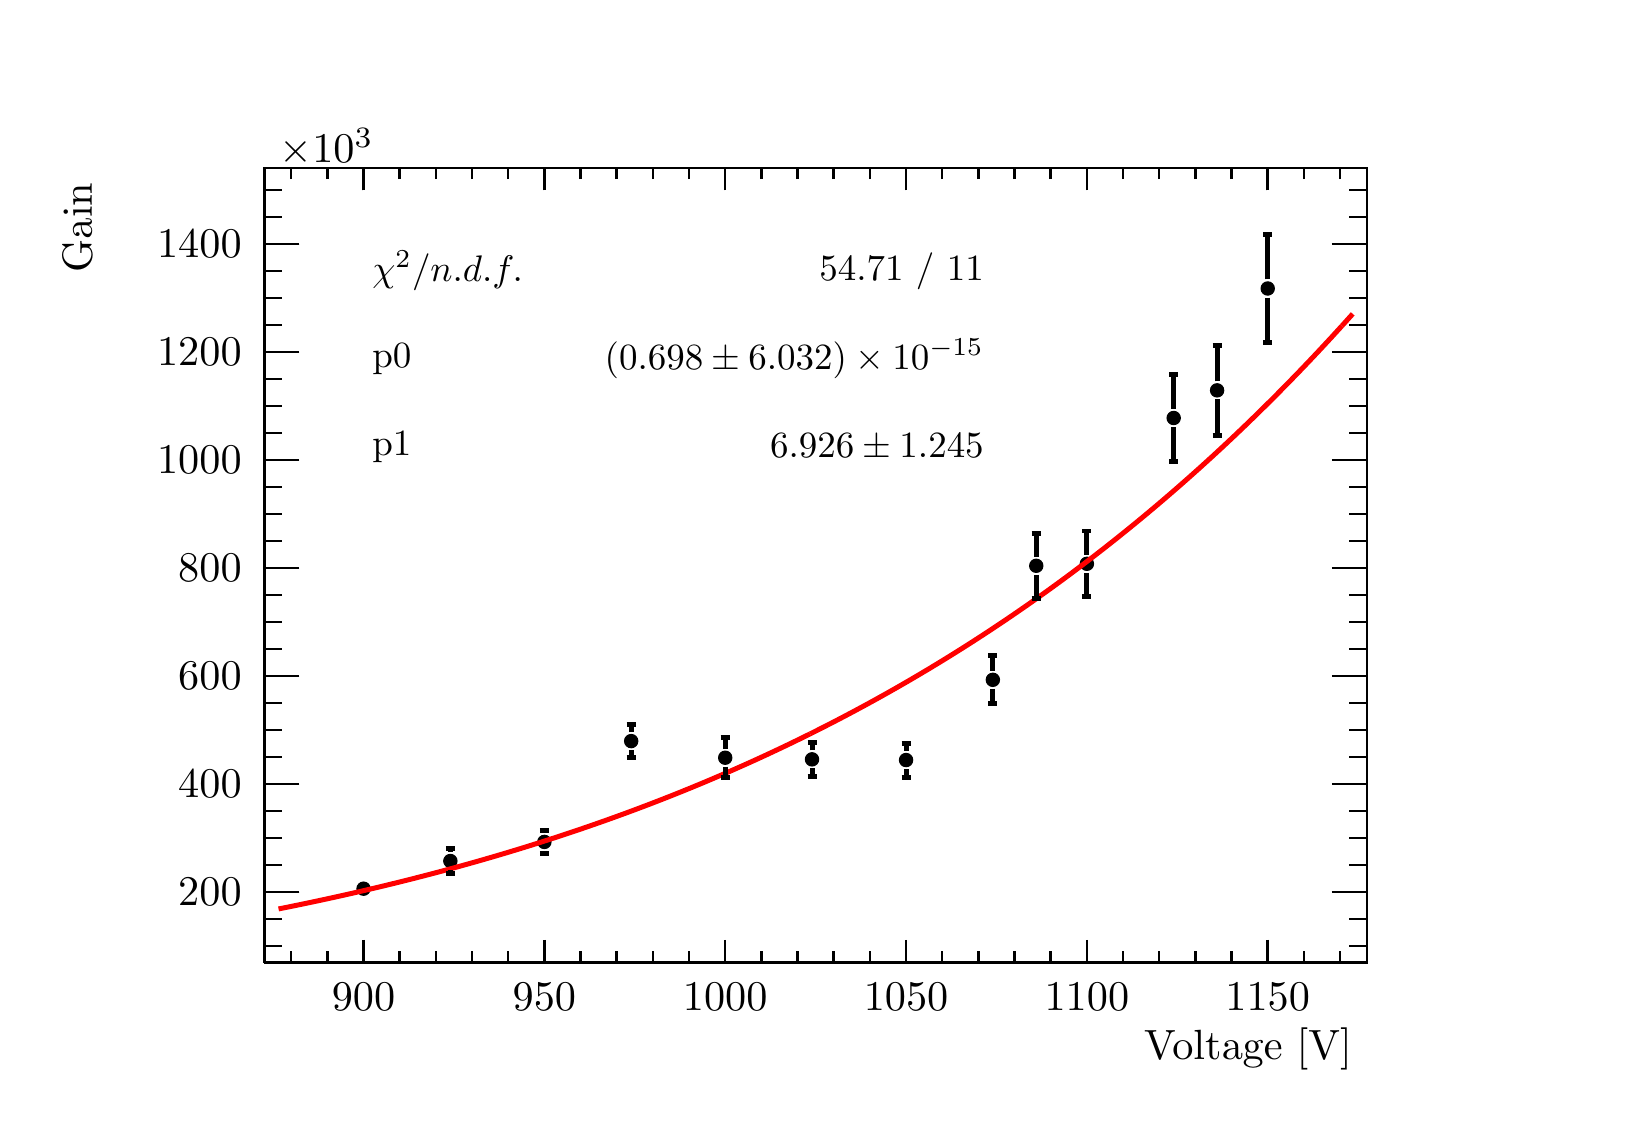
\begin{tikzpicture}
\pgfdeclareplotmark{cross} {
\pgfpathmoveto{\pgfpoint{-0.3\pgfplotmarksize}{\pgfplotmarksize}}
\pgfpathlineto{\pgfpoint{+0.3\pgfplotmarksize}{\pgfplotmarksize}}
\pgfpathlineto{\pgfpoint{+0.3\pgfplotmarksize}{0.3\pgfplotmarksize}}
\pgfpathlineto{\pgfpoint{+1\pgfplotmarksize}{0.3\pgfplotmarksize}}
\pgfpathlineto{\pgfpoint{+1\pgfplotmarksize}{-0.3\pgfplotmarksize}}
\pgfpathlineto{\pgfpoint{+0.3\pgfplotmarksize}{-0.3\pgfplotmarksize}}
\pgfpathlineto{\pgfpoint{+0.3\pgfplotmarksize}{-1.\pgfplotmarksize}}
\pgfpathlineto{\pgfpoint{-0.3\pgfplotmarksize}{-1.\pgfplotmarksize}}
\pgfpathlineto{\pgfpoint{-0.3\pgfplotmarksize}{-0.3\pgfplotmarksize}}
\pgfpathlineto{\pgfpoint{-1.\pgfplotmarksize}{-0.3\pgfplotmarksize}}
\pgfpathlineto{\pgfpoint{-1.\pgfplotmarksize}{0.3\pgfplotmarksize}}
\pgfpathlineto{\pgfpoint{-0.3\pgfplotmarksize}{0.3\pgfplotmarksize}}
\pgfpathclose
\pgfusepathqstroke
}
\pgfdeclareplotmark{cross*} {
\pgfpathmoveto{\pgfpoint{-0.3\pgfplotmarksize}{\pgfplotmarksize}}
\pgfpathlineto{\pgfpoint{+0.3\pgfplotmarksize}{\pgfplotmarksize}}
\pgfpathlineto{\pgfpoint{+0.3\pgfplotmarksize}{0.3\pgfplotmarksize}}
\pgfpathlineto{\pgfpoint{+1\pgfplotmarksize}{0.3\pgfplotmarksize}}
\pgfpathlineto{\pgfpoint{+1\pgfplotmarksize}{-0.3\pgfplotmarksize}}
\pgfpathlineto{\pgfpoint{+0.3\pgfplotmarksize}{-0.3\pgfplotmarksize}}
\pgfpathlineto{\pgfpoint{+0.3\pgfplotmarksize}{-1.\pgfplotmarksize}}
\pgfpathlineto{\pgfpoint{-0.3\pgfplotmarksize}{-1.\pgfplotmarksize}}
\pgfpathlineto{\pgfpoint{-0.3\pgfplotmarksize}{-0.3\pgfplotmarksize}}
\pgfpathlineto{\pgfpoint{-1.\pgfplotmarksize}{-0.3\pgfplotmarksize}}
\pgfpathlineto{\pgfpoint{-1.\pgfplotmarksize}{0.3\pgfplotmarksize}}
\pgfpathlineto{\pgfpoint{-0.3\pgfplotmarksize}{0.3\pgfplotmarksize}}
\pgfpathclose
\pgfusepathqfillstroke
}
\pgfdeclareplotmark{newstar} {
\pgfpathmoveto{\pgfqpoint{0pt}{\pgfplotmarksize}}
\pgfpathlineto{\pgfqpointpolar{44}{0.5\pgfplotmarksize}}
\pgfpathlineto{\pgfqpointpolar{18}{\pgfplotmarksize}}
\pgfpathlineto{\pgfqpointpolar{-20}{0.5\pgfplotmarksize}}
\pgfpathlineto{\pgfqpointpolar{-54}{\pgfplotmarksize}}
\pgfpathlineto{\pgfqpointpolar{-90}{0.5\pgfplotmarksize}}
\pgfpathlineto{\pgfqpointpolar{234}{\pgfplotmarksize}}
\pgfpathlineto{\pgfqpointpolar{198}{0.5\pgfplotmarksize}}
\pgfpathlineto{\pgfqpointpolar{162}{\pgfplotmarksize}}
\pgfpathlineto{\pgfqpointpolar{134}{0.5\pgfplotmarksize}}
\pgfpathclose
\pgfusepathqstroke
}
\pgfdeclareplotmark{newstar*} {
\pgfpathmoveto{\pgfqpoint{0pt}{\pgfplotmarksize}}
\pgfpathlineto{\pgfqpointpolar{44}{0.5\pgfplotmarksize}}
\pgfpathlineto{\pgfqpointpolar{18}{\pgfplotmarksize}}
\pgfpathlineto{\pgfqpointpolar{-20}{0.5\pgfplotmarksize}}
\pgfpathlineto{\pgfqpointpolar{-54}{\pgfplotmarksize}}
\pgfpathlineto{\pgfqpointpolar{-90}{0.5\pgfplotmarksize}}
\pgfpathlineto{\pgfqpointpolar{234}{\pgfplotmarksize}}
\pgfpathlineto{\pgfqpointpolar{198}{0.5\pgfplotmarksize}}
\pgfpathlineto{\pgfqpointpolar{162}{\pgfplotmarksize}}
\pgfpathlineto{\pgfqpointpolar{134}{0.5\pgfplotmarksize}}
\pgfpathclose
\pgfusepathqfillstroke
}
\definecolor{c}{rgb}{1,1,1};
\draw [color=c, fill=c] (0,0) rectangle (20,13.639);
\draw [color=c, fill=c] (3,1.77307) rectangle (17,11.8659);
\definecolor{c}{rgb}{0,0,0};
\draw [c,line width=0.9] (3,1.77307) -- (3,11.8659) -- (17,11.8659) -- (17,1.77307) -- (3,1.77307);
\definecolor{c}{rgb}{1,1,1};
\draw [color=c, fill=c] (3,1.77307) rectangle (17,11.8659);
\definecolor{c}{rgb}{0,0,0};
\draw [c,line width=0.9] (3,1.77307) -- (3,11.8659) -- (17,11.8659) -- (17,1.77307) -- (3,1.77307);
\draw [c,line width=0.9] (3,1.77307) -- (17,1.77307);
\draw [c,line width=0.9] (4.25853,2.05948) -- (4.25853,1.77307);
\draw [c,line width=0.9] (4.71785,1.91628) -- (4.71785,1.77307);
\draw [c,line width=0.9] (5.17717,1.91628) -- (5.17717,1.77307);
\draw [c,line width=0.9] (5.63648,1.91628) -- (5.63648,1.77307);
\draw [c,line width=0.9] (6.0958,1.91628) -- (6.0958,1.77307);
\draw [c,line width=0.9] (6.55512,2.05948) -- (6.55512,1.77307);
\draw [c,line width=0.9] (7.01444,1.91628) -- (7.01444,1.77307);
\draw [c,line width=0.9] (7.47375,1.91628) -- (7.47375,1.77307);
\draw [c,line width=0.9] (7.93307,1.91628) -- (7.93307,1.77307);
\draw [c,line width=0.9] (8.39239,1.91628) -- (8.39239,1.77307);
\draw [c,line width=0.9] (8.85171,2.05948) -- (8.85171,1.77307);
\draw [c,line width=0.9] (9.31102,1.91628) -- (9.31102,1.77307);
\draw [c,line width=0.9] (9.77034,1.91628) -- (9.77034,1.77307);
\draw [c,line width=0.9] (10.2297,1.91628) -- (10.2297,1.77307);
\draw [c,line width=0.9] (10.689,1.91628) -- (10.689,1.77307);
\draw [c,line width=0.9] (11.1483,2.05948) -- (11.1483,1.77307);
\draw [c,line width=0.9] (11.6076,1.91628) -- (11.6076,1.77307);
\draw [c,line width=0.9] (12.0669,1.91628) -- (12.0669,1.77307);
\draw [c,line width=0.9] (12.5262,1.91628) -- (12.5262,1.77307);
\draw [c,line width=0.9] (12.9856,1.91628) -- (12.9856,1.77307);
\draw [c,line width=0.9] (13.4449,2.05948) -- (13.4449,1.77307);
\draw [c,line width=0.9] (13.9042,1.91628) -- (13.9042,1.77307);
\draw [c,line width=0.9] (14.3635,1.91628) -- (14.3635,1.77307);
\draw [c,line width=0.9] (14.8228,1.91628) -- (14.8228,1.77307);
\draw [c,line width=0.9] (15.2822,1.91628) -- (15.2822,1.77307);
\draw [c,line width=0.9] (15.7415,2.05948) -- (15.7415,1.77307);
\draw [c,line width=0.9] (4.25853,2.05948) -- (4.25853,1.77307);
\draw [c,line width=0.9] (3.79921,1.91628) -- (3.79921,1.77307);
\draw [c,line width=0.9] (3.3399,1.91628) -- (3.3399,1.77307);
\draw [c,line width=0.9] (15.7415,2.05948) -- (15.7415,1.77307);
\draw [c,line width=0.9] (16.2008,1.91628) -- (16.2008,1.77307);
\draw [c,line width=0.9] (16.6601,1.91628) -- (16.6601,1.77307);
\draw [anchor=base] (4.25853,1.15931) node[scale=1.52731, color=c, rotate=0]{900};
\draw [anchor=base] (6.55512,1.15931) node[scale=1.52731, color=c, rotate=0]{950};
\draw [anchor=base] (8.85171,1.15931) node[scale=1.52731, color=c, rotate=0]{1000};
\draw [anchor=base] (11.1483,1.15931) node[scale=1.52731, color=c, rotate=0]{1050};
\draw [anchor=base] (13.4449,1.15931) node[scale=1.52731, color=c, rotate=0]{1100};
\draw [anchor=base] (15.7415,1.15931) node[scale=1.52731, color=c, rotate=0]{1150};
\draw [anchor= east] (17,0.681948) node[scale=1.52731, color=c, rotate=0]{ Voltage [V]};
\draw [c,line width=0.9] (3,11.8659) -- (17,11.8659);
\draw [c,line width=0.9] (4.25853,11.5795) -- (4.25853,11.8659);
\draw [c,line width=0.9] (4.71785,11.7227) -- (4.71785,11.8659);
\draw [c,line width=0.9] (5.17717,11.7227) -- (5.17717,11.8659);
\draw [c,line width=0.9] (5.63648,11.7227) -- (5.63648,11.8659);
\draw [c,line width=0.9] (6.0958,11.7227) -- (6.0958,11.8659);
\draw [c,line width=0.9] (6.55512,11.5795) -- (6.55512,11.8659);
\draw [c,line width=0.9] (7.01444,11.7227) -- (7.01444,11.8659);
\draw [c,line width=0.9] (7.47375,11.7227) -- (7.47375,11.8659);
\draw [c,line width=0.9] (7.93307,11.7227) -- (7.93307,11.8659);
\draw [c,line width=0.9] (8.39239,11.7227) -- (8.39239,11.8659);
\draw [c,line width=0.9] (8.85171,11.5795) -- (8.85171,11.8659);
\draw [c,line width=0.9] (9.31102,11.7227) -- (9.31102,11.8659);
\draw [c,line width=0.9] (9.77034,11.7227) -- (9.77034,11.8659);
\draw [c,line width=0.9] (10.2297,11.7227) -- (10.2297,11.8659);
\draw [c,line width=0.9] (10.689,11.7227) -- (10.689,11.8659);
\draw [c,line width=0.9] (11.1483,11.5795) -- (11.1483,11.8659);
\draw [c,line width=0.9] (11.6076,11.7227) -- (11.6076,11.8659);
\draw [c,line width=0.9] (12.0669,11.7227) -- (12.0669,11.8659);
\draw [c,line width=0.9] (12.5262,11.7227) -- (12.5262,11.8659);
\draw [c,line width=0.9] (12.9856,11.7227) -- (12.9856,11.8659);
\draw [c,line width=0.9] (13.4449,11.5795) -- (13.4449,11.8659);
\draw [c,line width=0.9] (13.9042,11.7227) -- (13.9042,11.8659);
\draw [c,line width=0.9] (14.3635,11.7227) -- (14.3635,11.8659);
\draw [c,line width=0.9] (14.8228,11.7227) -- (14.8228,11.8659);
\draw [c,line width=0.9] (15.2822,11.7227) -- (15.2822,11.8659);
\draw [c,line width=0.9] (15.7415,11.5795) -- (15.7415,11.8659);
\draw [c,line width=0.9] (4.25853,11.5795) -- (4.25853,11.8659);
\draw [c,line width=0.9] (3.79921,11.7227) -- (3.79921,11.8659);
\draw [c,line width=0.9] (3.3399,11.7227) -- (3.3399,11.8659);
\draw [c,line width=0.9] (15.7415,11.5795) -- (15.7415,11.8659);
\draw [c,line width=0.9] (16.2008,11.7227) -- (16.2008,11.8659);
\draw [c,line width=0.9] (16.6601,11.7227) -- (16.6601,11.8659);
\draw [c,line width=0.9] (3,1.77307) -- (3,11.8659);
\draw [c,line width=0.9] (3.444,2.67094) -- (3,2.67094);
\draw [c,line width=0.9] (3.222,3.01379) -- (3,3.01379);
\draw [c,line width=0.9] (3.222,3.35663) -- (3,3.35663);
\draw [c,line width=0.9] (3.222,3.69948) -- (3,3.69948);
\draw [c,line width=0.9] (3.444,4.04233) -- (3,4.04233);
\draw [c,line width=0.9] (3.222,4.38517) -- (3,4.38517);
\draw [c,line width=0.9] (3.222,4.72802) -- (3,4.72802);
\draw [c,line width=0.9] (3.222,5.07086) -- (3,5.07086);
\draw [c,line width=0.9] (3.444,5.41371) -- (3,5.41371);
\draw [c,line width=0.9] (3.222,5.75656) -- (3,5.75656);
\draw [c,line width=0.9] (3.222,6.0994) -- (3,6.0994);
\draw [c,line width=0.9] (3.222,6.44225) -- (3,6.44225);
\draw [c,line width=0.9] (3.444,6.78509) -- (3,6.78509);
\draw [c,line width=0.9] (3.222,7.12794) -- (3,7.12794);
\draw [c,line width=0.9] (3.222,7.47078) -- (3,7.47078);
\draw [c,line width=0.9] (3.222,7.81363) -- (3,7.81363);
\draw [c,line width=0.9] (3.444,8.15648) -- (3,8.15648);
\draw [c,line width=0.9] (3.222,8.49932) -- (3,8.49932);
\draw [c,line width=0.9] (3.222,8.84217) -- (3,8.84217);
\draw [c,line width=0.9] (3.222,9.18501) -- (3,9.18501);
\draw [c,line width=0.9] (3.444,9.52786) -- (3,9.52786);
\draw [c,line width=0.9] (3.222,9.8707) -- (3,9.8707);
\draw [c,line width=0.9] (3.222,10.2136) -- (3,10.2136);
\draw [c,line width=0.9] (3.222,10.5564) -- (3,10.5564);
\draw [c,line width=0.9] (3.444,10.8992) -- (3,10.8992);
\draw [c,line width=0.9] (3.444,2.67094) -- (3,2.67094);
\draw [c,line width=0.9] (3.222,2.3281) -- (3,2.3281);
\draw [c,line width=0.9] (3.222,1.98525) -- (3,1.98525);
\draw [c,line width=0.9] (3.444,10.8992) -- (3,10.8992);
\draw [c,line width=0.9] (3.222,11.2421) -- (3,11.2421);
\draw [c,line width=0.9] (3.222,11.5849) -- (3,11.5849);
\draw [anchor= east] (2.9,2.67094) node[scale=1.52731, color=c, rotate=0]{200};
\draw [anchor= east] (2.9,4.04233) node[scale=1.52731, color=c, rotate=0]{400};
\draw [anchor= east] (2.9,5.41371) node[scale=1.52731, color=c, rotate=0]{600};
\draw [anchor= east] (2.9,6.78509) node[scale=1.52731, color=c, rotate=0]{800};
\draw [anchor= east] (2.9,8.15648) node[scale=1.52731, color=c, rotate=0]{1000};
\draw [anchor= east] (2.9,9.52786) node[scale=1.52731, color=c, rotate=0]{1200};
\draw [anchor= east] (2.9,10.8992) node[scale=1.52731, color=c, rotate=0]{1400};
\draw [anchor=base west] (3,11.9341) node[scale=1.52731, color=c, rotate=0]{$\times10^{3}$};
\draw [anchor= east] (0.624642,11.8659) node[scale=1.52731, color=c, rotate=90]{ Gain};
\draw [c,line width=0.9] (17,1.77307) -- (17,11.8659);
\draw [c,line width=0.9] (16.556,2.67094) -- (17,2.67094);
\draw [c,line width=0.9] (16.778,3.01379) -- (17,3.01379);
\draw [c,line width=0.9] (16.778,3.35663) -- (17,3.35663);
\draw [c,line width=0.9] (16.778,3.69948) -- (17,3.69948);
\draw [c,line width=0.9] (16.556,4.04233) -- (17,4.04233);
\draw [c,line width=0.9] (16.778,4.38517) -- (17,4.38517);
\draw [c,line width=0.9] (16.778,4.72802) -- (17,4.72802);
\draw [c,line width=0.9] (16.778,5.07086) -- (17,5.07086);
\draw [c,line width=0.9] (16.556,5.41371) -- (17,5.41371);
\draw [c,line width=0.9] (16.778,5.75656) -- (17,5.75656);
\draw [c,line width=0.9] (16.778,6.0994) -- (17,6.0994);
\draw [c,line width=0.9] (16.778,6.44225) -- (17,6.44225);
\draw [c,line width=0.9] (16.556,6.78509) -- (17,6.78509);
\draw [c,line width=0.9] (16.778,7.12794) -- (17,7.12794);
\draw [c,line width=0.9] (16.778,7.47078) -- (17,7.47078);
\draw [c,line width=0.9] (16.778,7.81363) -- (17,7.81363);
\draw [c,line width=0.9] (16.556,8.15648) -- (17,8.15648);
\draw [c,line width=0.9] (16.778,8.49932) -- (17,8.49932);
\draw [c,line width=0.9] (16.778,8.84217) -- (17,8.84217);
\draw [c,line width=0.9] (16.778,9.18501) -- (17,9.18501);
\draw [c,line width=0.9] (16.556,9.52786) -- (17,9.52786);
\draw [c,line width=0.9] (16.778,9.8707) -- (17,9.8707);
\draw [c,line width=0.9] (16.778,10.2136) -- (17,10.2136);
\draw [c,line width=0.9] (16.778,10.5564) -- (17,10.5564);
\draw [c,line width=0.9] (16.556,10.8992) -- (17,10.8992);
\draw [c,line width=0.9] (16.556,2.67094) -- (17,2.67094);
\draw [c,line width=0.9] (16.778,2.3281) -- (17,2.3281);
\draw [c,line width=0.9] (16.778,1.98525) -- (17,1.98525);
\draw [c,line width=0.9] (16.556,10.8992) -- (17,10.8992);
\draw [c,line width=0.9] (16.778,11.2421) -- (17,11.2421);
\draw [c,line width=0.9] (16.778,11.5849) -- (17,11.5849);
\foreach \P in {(4.25853,2.71105), (5.36089,3.06272), (6.55512,3.30505), (7.65748,4.5854), (8.85171,4.37434), (9.95407,4.35366), (11.1483,4.34486), (12.2507,5.36374), (12.8018,6.81202), (13.4449,6.83732), (14.5472,8.68883), (15.0984,9.03984),
 (15.7415,10.3335)}{\draw[mark options={color=c,fill=c},mark size=2.402402pt,mark=*] plot coordinates {\P};}
\definecolor{c}{rgb}{1,0,0};
\draw [c,line width=1.8] (3.17913,2.45386) -- (3.31693,2.4815) -- (3.45472,2.50971) -- (3.59252,2.53849) -- (3.73031,2.56786) -- (3.86811,2.59782) -- (4.00591,2.62838) -- (4.1437,2.65956) -- (4.2815,2.69136) -- (4.41929,2.72379) -- (4.55709,2.75687)
 -- (4.69488,2.7906) -- (4.83268,2.825) -- (4.97047,2.86008) -- (5.10827,2.89584) -- (5.24606,2.93231) -- (5.38386,2.96948) -- (5.52165,3.00738) -- (5.65945,3.04601) -- (5.79724,3.08538) -- (5.93504,3.12551) -- (6.07283,3.16641) -- (6.21063,3.2081)
 -- (6.34843,3.25057) -- (6.48622,3.29385) -- (6.62402,3.33796) -- (6.76181,3.38289) -- (6.89961,3.42867) -- (7.0374,3.4753) -- (7.1752,3.52281) -- (7.31299,3.5712) -- (7.45079,3.62049) -- (7.58858,3.67069) -- (7.72638,3.72182) -- (7.86417,3.77389)
 -- (8.00197,3.82691) -- (8.13976,3.88091) -- (8.27756,3.93588) -- (8.41535,3.99186) -- (8.55315,4.04885) -- (8.69094,4.10687) -- (8.82874,4.16593) -- (8.96654,4.22605) -- (9.10433,4.28725) -- (9.24213,4.34954) -- (9.37992,4.41294) --
 (9.51772,4.47746) -- (9.65551,4.54312) -- (9.79331,4.60994) -- (9.9311,4.67794);
\draw [c,line width=1.8] (9.9311,4.67794) -- (10.0689,4.74712) -- (10.2067,4.81752) -- (10.3445,4.88914) -- (10.4823,4.962) -- (10.6201,5.03613) -- (10.7579,5.11154) -- (10.8957,5.18824) -- (11.0335,5.26627) -- (11.1713,5.34562) -- (11.3091,5.42633)
 -- (11.4469,5.50842) -- (11.5846,5.5919) -- (11.7224,5.67679) -- (11.8602,5.76311) -- (11.998,5.85089) -- (12.1358,5.94014) -- (12.2736,6.03088) -- (12.4114,6.12314) -- (12.5492,6.21693) -- (12.687,6.31228) -- (12.8248,6.4092) -- (12.9626,6.50772)
 -- (13.1004,6.60787) -- (13.2382,6.70966) -- (13.376,6.81311) -- (13.5138,6.91825) -- (13.6516,7.0251) -- (13.7894,7.13369) -- (13.9272,7.24403) -- (14.065,7.35615) -- (14.2028,7.47008) -- (14.3406,7.58584) -- (14.4783,7.70345) -- (14.6161,7.82294)
 -- (14.7539,7.94433) -- (14.8917,8.06765) -- (15.0295,8.19291) -- (15.1673,8.32016) -- (15.3051,8.44942) -- (15.4429,8.5807) -- (15.5807,8.71404) -- (15.7185,8.84947) -- (15.8563,8.98701) -- (15.9941,9.12668) -- (16.1319,9.26852) --
 (16.2697,9.41255) -- (16.4075,9.55881) -- (16.5453,9.70732) -- (16.6831,9.8581);
\draw [c,line width=1.8] (16.6831,9.8581) -- (16.8209,10.0112);
\definecolor{c}{rgb}{1,1,1};
\draw [color=c, fill=c] (3.75358,7.76504) rectangle (12.7507,11.1175);
\definecolor{c}{rgb}{0,0,0};
\draw [anchor= west] (4.20344,10.5587) node[scale=1.3364, color=c, rotate=0]{$\chi^{2} / \text{n.d.f.} $};
\draw [anchor= east] (12.3009,10.5587) node[scale=1.3364, color=c, rotate=0]{ 54.71 / 11};
\draw [anchor= west] (4.20344,9.44126) node[scale=1.3364, color=c, rotate=0]{p0       };
\draw [anchor= east] (12.3009,9.44126) node[scale=1.3364, color=c, rotate=0]{$ \num{6.978d-16} \pm \num{6.032d-15}$};
\draw [anchor= west] (4.20344,8.32378) node[scale=1.3364, color=c, rotate=0]{p1       };
\draw [anchor= east] (12.3009,8.32378) node[scale=1.3364, color=c, rotate=0]{$ 6.926 \pm 1.245$};
\draw [c,line width=1.8] (5.36089,3.17734) -- (5.36089,3.2271);
\draw [c,line width=1.8] (5.30359,3.2271) -- (5.4182,3.2271);
\draw [c,line width=1.8] (5.36089,2.94811) -- (5.36089,2.89834);
\draw [c,line width=1.8] (5.30359,2.89834) -- (5.4182,2.89834);
\draw [c,line width=1.8] (6.55512,3.41967) -- (6.55512,3.44871);
\draw [c,line width=1.8] (6.49781,3.44871) -- (6.61242,3.44871);
\draw [c,line width=1.8] (6.55512,3.19044) -- (6.55512,3.1614);
\draw [c,line width=1.8] (6.49781,3.1614) -- (6.61242,3.1614);
\draw [c,line width=1.8] (7.65748,4.70001) -- (7.65748,4.79579);
\draw [c,line width=1.8] (7.60017,4.79579) -- (7.71479,4.79579);
\draw [c,line width=1.8] (7.65748,4.47078) -- (7.65748,4.375);
\draw [c,line width=1.8] (7.60017,4.375) -- (7.71479,4.375);
\draw [c,line width=1.8] (8.85171,4.48895) -- (8.85171,4.63068);
\draw [c,line width=1.8] (8.7944,4.63068) -- (8.90901,4.63068);
\draw [c,line width=1.8] (8.85171,4.25973) -- (8.85171,4.118);
\draw [c,line width=1.8] (8.7944,4.118) -- (8.90901,4.118);
\draw [c,line width=1.8] (9.95407,4.46827) -- (9.95407,4.57027);
\draw [c,line width=1.8] (9.89676,4.57027) -- (10.0114,4.57027);
\draw [c,line width=1.8] (9.95407,4.23905) -- (9.95407,4.13706);
\draw [c,line width=1.8] (9.89676,4.13706) -- (10.0114,4.13706);
\draw [c,line width=1.8] (11.1483,4.45948) -- (11.1483,4.56081);
\draw [c,line width=1.8] (11.091,4.56081) -- (11.2056,4.56081);
\draw [c,line width=1.8] (11.1483,4.23025) -- (11.1483,4.12891);
\draw [c,line width=1.8] (11.091,4.12891) -- (11.2056,4.12891);
\draw [c,line width=1.8] (12.2507,5.47835) -- (12.2507,5.6703);
\draw [c,line width=1.8] (12.1933,5.6703) -- (12.308,5.6703);
\draw [c,line width=1.8] (12.2507,5.24913) -- (12.2507,5.05718);
\draw [c,line width=1.8] (12.1933,5.05718) -- (12.308,5.05718);
\draw [c,line width=1.8] (12.8018,6.92663) -- (12.8018,7.22262);
\draw [c,line width=1.8] (12.7445,7.22262) -- (12.8591,7.22262);
\draw [c,line width=1.8] (12.8018,6.6974) -- (12.8018,6.40141);
\draw [c,line width=1.8] (12.7445,6.40141) -- (12.8591,6.40141);
\draw [c,line width=1.8] (13.4449,6.95193) -- (13.4449,7.25373);
\draw [c,line width=1.8] (13.3876,7.25373) -- (13.5022,7.25373);
\draw [c,line width=1.8] (13.4449,6.7227) -- (13.4449,6.4209);
\draw [c,line width=1.8] (13.3876,6.4209) -- (13.5022,6.4209);
\draw [c,line width=1.8] (14.5472,8.80345) -- (14.5472,9.24699);
\draw [c,line width=1.8] (14.4899,9.24699) -- (14.6046,9.24699);
\draw [c,line width=1.8] (14.5472,8.57422) -- (14.5472,8.13068);
\draw [c,line width=1.8] (14.4899,8.13068) -- (14.6046,8.13068);
\draw [c,line width=1.8] (15.0984,9.15446) -- (15.0984,9.614);
\draw [c,line width=1.8] (15.0411,9.614) -- (15.1557,9.614);
\draw [c,line width=1.8] (15.0984,8.92523) -- (15.0984,8.46569);
\draw [c,line width=1.8] (15.0411,8.46569) -- (15.1557,8.46569);
\draw [c,line width=1.8] (15.7415,10.4481) -- (15.7415,11.0248);
\draw [c,line width=1.8] (15.6842,11.0248) -- (15.7988,11.0248);
\draw [c,line width=1.8] (15.7415,10.2189) -- (15.7415,9.64217);
\draw [c,line width=1.8] (15.6842,9.64217) -- (15.7988,9.64217);
\definecolor{c}{rgb}{1,1,1};
\draw [color=c, fill=c] (3.75358,7.76504) rectangle (12.7507,11.1175);
\definecolor{c}{rgb}{0,0,0};
\draw [anchor= west] (4.20344,10.5587) node[scale=1.3364, color=c, rotate=0]{$\chi^{2} / \text{n.d.f.} $};
\draw [anchor= east] (12.3009,10.5587) node[scale=1.3364, color=c, rotate=0]{ 54.71 / 11};
\draw [anchor= west] (4.20344,9.44126) node[scale=1.3364, color=c, rotate=0]{p0       };
\draw [anchor= east] (12.3009,9.44126) node[scale=1.3364, color=c, rotate=0]{$ (0.698 \pm 6.032) \times 10^{-15}$};
\draw [anchor= west] (4.20344,8.32378) node[scale=1.3364, color=c, rotate=0]{p1       };
\draw [anchor= east] (12.3009,8.32378) node[scale=1.3364, color=c, rotate=0]{$ 6.926 \pm 1.245$};
\definecolor{c}{rgb}{1,1,1};
\draw [color=c, fill=c] (2,12.8206) rectangle (18,13.5708);
\definecolor{c}{rgb}{0,0,0};
%\draw (10,13.1957) node[scale=1.20912, color=c, rotate=0]{PMT gain with varying voltage (PMT 0446, 1.5V amp., 1.5V offset)};
\end{tikzpicture}

  \end{adjustbox}
  \caption[Example of relationship between PMT voltage and gain]{An example of the relationship between PMT voltage and gain. A curve of the form $p_{0} V^{p_{1}}$ is fitted and shown in red.}
  \label{fig:gainEx}
\end{figure}

\subsection{Bar timing resolution measurements}
\label{ch:hptpc_dtof_characterisation:characterisation:barRes}

In order to measure the time and position resolution of the bars, the PMTs are attached to the bars as stated in \citesec{ch:hptpc_dtof_characterisation:dtof}.
Following this, the bars are placed into a light-tight box to ensure that the PMTs do not observe light from outside sources.

A $\text{Sr}^{90}$ source is the primary tool used to evaluate the time and position resolution of the bars.
$\text{Sr}^{90}$ decays almost entirely via $\beta$-decay with an end-point of \SI{0.546}{\mega\electronvolt} to $\text{Y}^{90}$ which itself decays via $\beta$-decay with an end-point of \SI{2.28}{\mega\electronvolt}~\cite{strontium}.
